
\documentclass{InsightArticle}


%%%%%%%%%%%%%%%%%%%%%%%%%%%%%%%%%%%%%%%%%%%%%%%%%%%%%%%%%%%%%%%%%%
%
%  hyperref should be the last package to be loaded.
%
%%%%%%%%%%%%%%%%%%%%%%%%%%%%%%%%%%%%%%%%%%%%%%%%%%%%%%%%%%%%%%%%%%
\usepackage[dvips,
bookmarks,
bookmarksopen,
backref,
colorlinks,linkcolor={blue},citecolor={blue},urlcolor={blue},
]{hyperref}
\usepackage{graphicx}
\usepackage{listings}
\usepackage{subfigure}
\usepackage{pseudocode}
% \usepackage{algorithm}
% \usepackage{algorithmic}


\title{The watershed transform in ITK - discussion and new developments}

%\release{1.00}

\author{Richard Beare{$^1$} {\small{and}} Ga\"etan Lehmann{$^2$}}
\authoraddress{{$^1$}Department of Medicine, Moansh University, Australia.\\ 
{$^2$}Unit\'e de Biologie du D\'eveloppement et de la Reproduction, Institut National de la Recherche Agronomique, 78350 Jouy-en-Josas, France}


\begin{document}
\maketitle

\ifhtml
\chapter*{Front Matter\label{front}}
\fi


\begin{abstract}
\noindent
This report discusses various definitions and implementations of the
watershed transform as well as providing an introduction to some well
known techniques for applying the watershed transform to practical
problems. The discussion will be focussed on new and existing ITK
classes.
\end{abstract}

\tableofcontents
\section{Introduction}

The watershed transform is a tool for image segmentation that is fast
and flexible and potentially fairly parameter free. It was originally
derived from a geophysical model of rain falling on a terrain and a variety
of more formal definitions have been devised to allow development of
practical algorithms. A brief discussion of some of these definitions
and algorithms is provided in Section \ref{sect:history}. 

Section \ref{sect:usingWT} provides an introduction to a
methodology known as {\em marker based} watershed. Using markers in
watershed transforms is a well established technique in the
morphological image analysis community and has proved very useful for
many applications. The aim of this part of the report is to describe
the technique to a wider audience \footnote{It should also be noted
that the lack of a marker based watershed motivated the recent work on
ITK filter classes.}.

A brief description of two algorithms used to implement the watershed
transform is given in Section \ref{sect:algorithms}.

\section{Image segmentation}
Image segmentation, in the context of this report, may be broadly
defined as finding the part(s) of the image that is of interest in
order to make measurements. This is a basic definition of image
analysis, which is different from image processing and computer
vision\footnote{Image processing produces images, usually for human
consumption, while computer vision aims to produce high level semantic
descriptions of images.}.

It is very rare to achieve a useful segmentation using a single
procedure, even under the most favourable conditions. Successful
segmentation algorithms typically use a carefully constructed
combination of procedures to achieve useful results. Some modern
algorithms, especially the family of routines related to geodesic
active contours, may seem to be an exception to this rule of thumb
because they are often presented as achieving good segmentation
results entirely on their own. However close examination will show
that a variety of preprocessing steps in addition to careful parameter
tuning is necessary to achieve anything useful.

These comments are also relevant to the watershed transform -- it is
very unlikely that any segmentation problem can be solved using the
watershed alone. However it is a very useful and flexible tool that
can be applied in a number of ways. This report will emphasise the
marker based approach to using the watershed transform, but there are
a number of others including watershed trees and region merging
algorithms.

Finally, an important point that should be mentioned, is that the
output of a low level segmentation procedure such as the watershed
transform will typically be a {\em label image}. A label image,
sometimes referred to as a categorical image, has unique values for
each region. For example, if a watershed produces 2 regions, all
pixels belonging to one region would have value $A$, and all belonging
to the other might have value $B$. Unassigned pixels, such as
watershed lines, might have value of $0$.

\section{The watershed transform -- a brief history}
\label{sect:history}
The watershed transform was first proposed by Beucher and
Lantu\'{e}joul\cite{Beucher-Lantu-79} as a geophysical model of rain
falling on a terrain. The idea is that a raindrop falling on a surface
will trickle down the path of steepest descent to a minima. The set of
points on the surface that lead to the same minima is known as a
catchment basin and borders between catchment basins are watershed
lines\footnote{Major geographical features, like rivers or oceans, are
often considered as separated by watershed lines, usually along
mountain ranges.}. If an image is considered as a terrain and divided
into catchment basins then the hope is that each catchment basin would
contain an object of interest. The image representing the terrain will
be referred to as the {\em control surface} in this report.

Translating the model of rain falling on a terrain to an algorithm has
a number of problems\footnote{Although this is what the first ITK
implementation does.} which are discussed in Section
\ref{sect:rainfallmodel}. The alternative is to imagine a flooding
process, with each regional minima\footnote{A regional minima is a set
of pixels surrounded by pixels of higher value.} becoming the source
of a lake. The terrain is progressively flooded and lakes eventually
meet neighboring lakes. Virtual dams are constructed to keep the
neighboring lakes separate as the waterlevel rises. When the image
surface is completely fooded the virtual dams correspond to the
watershed lines\footnote{In 3D neighboring lakes meet at surfaces.}.

A major breakthrough in the implementation of the watershed was made
by Vincent and Soille \cite{Vincent91a} with the introduction of the
first queue based implementation of the watershed transform. This was
especially significant because it allowed similar execution times on
conventional computer systems as was being achieved with specialized
parallel processing systems. The Vincent-Soille algorithm appears to
be used in the matlab image processing toolbox watershed
implementation (based on the observation that the library function has
a {\tt \_vs} suffix).

Another major advance made soon after by Meyer and Beucher
\cite{Beucher93a,Meyer1994a}. Meyer defined the watershed transform in terms of {\em
topographic distances} through {\em lower complete} images. These
definitions rigorously defined the behavior in the presence of
plateaus and lead to some new algorithms based on graph theory. Two
examples of these algorithms are {\em hill-climbing} and {\em image
integration} and will be discussed in more detail in this report.


Readers interested in more technical detail should refer to \cite{Roerdink2000a,Meijster2004a}.

\subsection{The topological watershed}
An alternative approach, known as the topological watershed, has
recently been developed \cite{}. The topological watershed modifies
the topology of the surface so that all pixels that are not watershed
lines become regional minima and watershed lines are modified so that
they are more suitable for use in measuring saliency of boundaries
between regions. Algorithms implementing the topological watershed
also exploit priority queues, but don't appear to be able to avoid the
need for explicit lower completion or reconstruction by erosion.

The topological watershed appears to have been developed with the aim
of using measures of border significance for merging criteria. This
work lead to the discovery that it wasn't possible to compute certain
measures with the flooding approaches used by many implementations.

I don't understand the implications of the topological watershed yet.

\section{Rainfall model}
\label{sect:rainfall}
{\em where should we put this?}  The original concept behind the
watershed transform was rain falling on a terrain and flowing down
paths of steepest descent to local minima. There has been a lot of
work on alternatives to this approach because of the problems with
it. These problems are basically to do with flat zones in an image
which have no paths of steepest descent leading from them, which means
that water would just sit in the one spot. A simple minded
implementation of this idea would therefore produce a separate
catchment basin for each pixel in the flat zone, which is not a very
useful result. The ITK watershed uses a number of steps to avoid this problem:
\begin{enumerate}
\item Label all minima and flat zones.
\item Trace all unlabelled pixels to a labelled one using gradient descent.
\item Check each flat region and find the lowest neighbor. Change the label of the flat region to that of the lowest neighbor.
\end{enumerate}
 
It should be evident that a number of arbitary choices have been made
here - for example it is impossible to break a flat region into
pieces, which would probably better fit the physical reality of
rainfall (consider a flat topped ridge which should perhaps be split
down the middle). What happens of there are multiple neighboring
regions with equal height - is the labelling decision now somewhat arbitary?

In general the flooding models avoid these dilemas and lead to more
elegant algorithms.


\section{Using the watershed tranform}
\label{sect:usingWT}
\subsection{Classical approach}
The simplest way of using the watershed is to preprocess the image we
want to segment so that the boundaries of our objects are bright (e.g
apply an edge detector) and compute the watershed transform of the
edge image. Watershed lines will correspond to the boundaries and our
problem will be solved. This is rarely useful in practice because
there are always more regional minima than there are objects, either
due to noise or natural variations in the object surfaces. Therefore,
while many watershed lines do lie on significant boundaries, there are
many that don't. Figure \ref{fig:overseg} illustrates the problem. The ITK
watershed implementation provides a way of addressing this problem
using a measure of significance of the boundary and allowing a
threshold to be applied first to reduce the number of local minima. 

An Obvious alternative that is very similar in practice is to 
smooth the image so that there are fewer regional minima.
\begin{figure}
\begin{center}
\caption{Classical over segmentation.}
\label{fig:overseg}
\end{center}
\end{figure}

There are some situations where this direct approach can be
useful. The best known of these is probably binary object splitting,
in which the watershed transform is applied to the distance transform
of a mask. This approach is widely used to split touching,
approximately circular objects, such as cells.

\subsection{Watershed from selected minima}
An alternative approach leads us to the concept of markers mentioned
earlier. We will also see that the thresholding approach used by ITK
may be considered as a specific case of the same approach.

Suppose we have preprocessing steps that let select regional minima
that lead to the correct segmentation. How would we modify the
topography of the image so that only the desired regional minima are
present and the watershed lines that remain are the same as they were
before the modification (i.e we only remove the unwanted boundaries)?

This can be achieved by performing a {\em reconstruction by erosion}
or {\em recursive conditional erosion} from the seleted regional
minima. Figure \ref{fig:recon} illustrates the results of apply a
reconstruction by erosion to a 1D image. The original image is shown
in blue and has regional minima A, B, C, D and E. The marker image
which is recursively eroded is shown in black, with a single zero at
regional minimum B. The red plateaus illustrate the parts of the
result image that are above the orginal. The resulting image has only
on regional minima that corresponds to B.
\begin{figure}[htbp]
\begin{center}
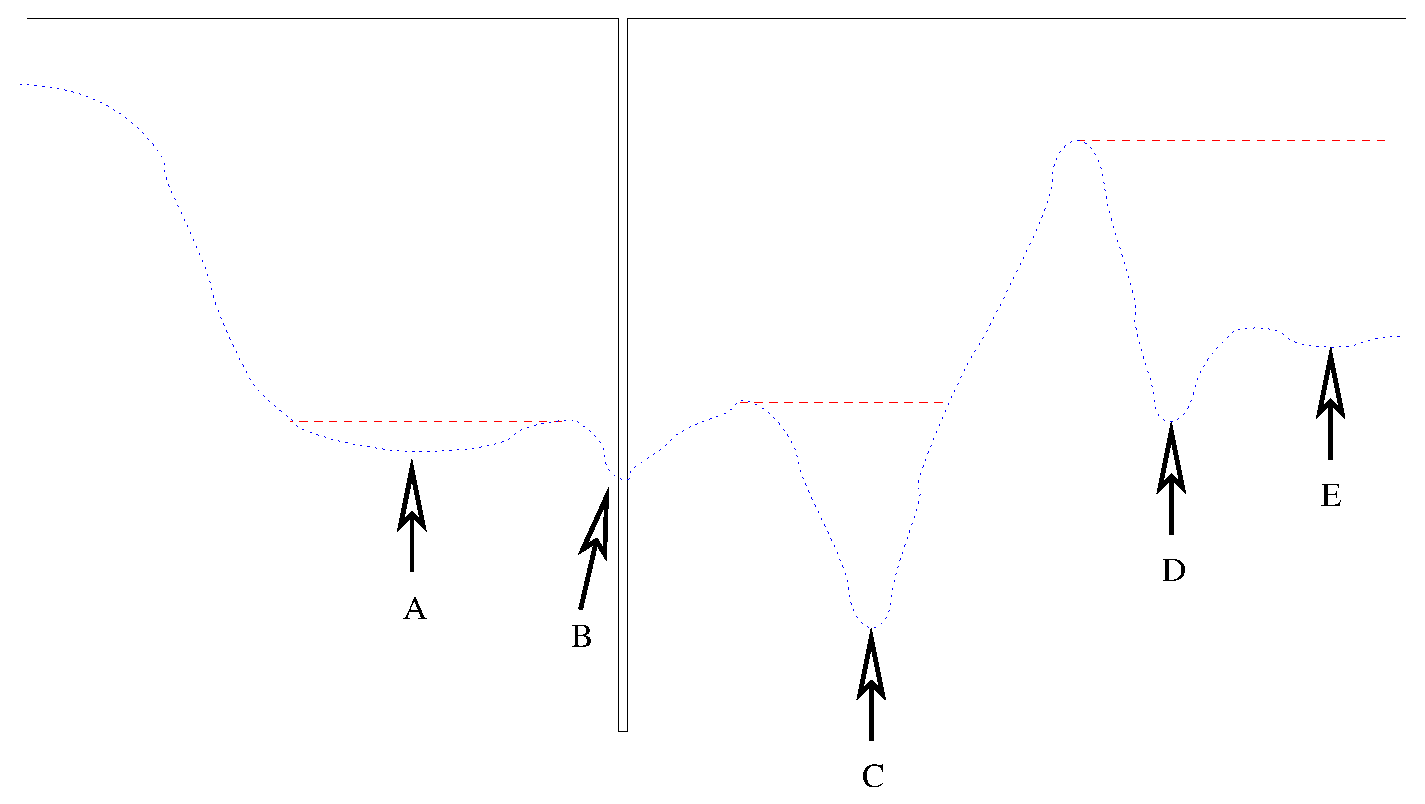
\includegraphics[scale=0.5]{recon}
\caption{Reconstruction by erosion from a single regional minimum.}
\label{fig:recon}
\end{center}
\end{figure}

A more formal definition of recursive erosion is:
\begin{equation}
\label{eq:recon_erosion}
h_{n+1}=\max\{f, \varepsilon h_n\}
\end{equation}
where $h_0(x)$ is the function, with value 0 at the markers and
$\infty$ otherwise and $\varepsilon$ denotes the erosion
operation.

This procedure may not seem to offer much advantage -- after all how
are we going to decide which minima are useful to us? The key step to
using these ideas in practice is to realize that an arbitary mask
image can be used to create minima in an image in locations we want
simply by multiplying the image by the mask. Recursive erosion of the
original image using that mask then produces a topology to which we
can apply a watershed transform. The mask image is commonly called a
marker image.

This is the fundamental concept behind the use of markers in watershed
based segmentation.

Let's summarize the steps again:

\begin{enumerate}
\item Generate a marker image. The marker image will be used to create 
one, possibly extended, minima inside each object of interest. A
marker image will always need to create at least two minima, and at
least one minima will probably be used to segment the background. The
marker image may be generated via interaction with an operator or by
various preprocessing steps.
\item \label{recipe:min}Impose the minima on the control surface. This 
might be done by multiplying by the marker image (or an inverted
version of it, depending on convention).
\item \label{recipe:erode}Recursively erode the control surface to eliminate all minima besides those introduced in the previous step. This produces a new control surface.
\item Apply the watershed tranform to the new surface.
\end{enumerate}

\subsection{Efficiency issues}
The procedure outlined above introduces a lot of additional steps,
some of which could be reasonably computationally expensive
(i.e. recursive erosion). Other steps have also been mentioned in
passing ({\em lower completion} in Section \ref{sect:history} that may
be potentially time consuming. Fortunately we will discover in Section
\ref{sect:algorithms} that the appropriate choice of algorithm implementing the
watershed transform will carry out these steps implicitly.

\section{Algorithms}
\label{sect:algorithms}
The two that will be outlined here are known as {\em image
integration}\cite{Meyer1994a} and {\em hill climbing}
\cite{Beucher93a}, both of which are classed as ordered
algorithms and are examples of graph flooding approaches. These
algorithms implement the watershed tranform by topographic distance
(or approximate it) and are derived from Dijkstra-Moore minimal path
algorithms of graph theory.

\subsection{Ordered queues}
Both of these implementations depend on ordered queues to avoid the
need for explicit computation of lower complete images and recursive
erosion. An ordered queue is a heirarchical priority queue with two
levels. One level is defined by the pixel gray level, with darker
pixels having higher priority, while the second applies to pixels of
the same grey level and provides a FIFO ordering. The FIFO ordering
leads to a breadth first propogation across plateaus because the
ordering becomes related to distance from the regional minima. This is
the mechanism that avoids the to explicitly compute lower slope.

Early implementations used a special ordered queue for 8 bit data,
which may be where the misconception that a morphological watershed
can only be applied to 8 bit data types arose -- in fact some of the
early work along these lines was covered by a patent\footnote{I'm told
that the associated paper is \cite{Meyer91a} and that there may be an
English version in \cite{Dougherty93a}}. The new ITK watershed
algorithms use standard c++ containers (maps and standard queues) to
implement the ordered queue\footnote{One potential problem with
applying this style of algorithm to non integer data is finding the
regional minima. Reconstruction approaches are often used to find
regional minima of integer type images, but subtracting 1, carrying
out a recursive dilation and subtracting the two. The same concept
does not extend to floating point data. However, if regional minima
are available the algorithms we are discussing can be applied to
floating point data.}.

In both algorithms each pixel is regarded as a node in a graph that is
connected to neighboring pixels by pairs of edges. Costs of the edges
are defined in terms of a cost related to the gradient.

\subsection{Image integration}
This algorithm maintains a pair of images -- a distance image and a
label image. The distance image is initialized to initialized to
$\infty$ everywhere, except at the minima where it is initialized to
the value of the minima while the label image is initialized to $0$
everywhere, except at the minima where it is initialized to the index
of the minima (or, more typically, the value of the marker image at
those points).

Wavefronts are propogated from each minima, using the ordered queue
approach. As the wavefront reaches pixel the distance travelled by the
wavefront is compared to the distance stored in the distance image. If
the distance travelled by the new wavefront is less than the stored
value then that pixel is given the label associated with the
wavefront, otherwise the label is left unchanged.

\subsection{Hill climbing}
Hill climbing is an approximation that eliminates the need to maintain
a distance image. The approximation employed is that distances between
all neighbors in a 4, 6, 8, 18 or 26\footnote{4 and 8 connected
neighborhoods are used in 2D, 6, 18 and 26 in 3D} and the center of
the neighborhood are equal -- i.e the various $\sqrt{2}$ terms are
ignored. The position of the watershed lines can have some dependence
on raster ordering because of this. In general the approach is very
useful and efficient.

There seem to be at least 3 algorithms that fall into the
hill-climbing category.

%Hill climbing requires a label image which is initialized to the
%indexes of the regional minima at the regional minima and an UNKNOWN
%value elsewhere\footnote{In the ITK implementation a separate image is
%used to track UNKNOWN locations because UNKNOWN values are difficult
%to deal with in a type independent way.}. The priority queue is
%initialised with the borders of the regional minima. Pixels pushed
%onto the queue with priority defined by their grey level and labelled
%as they are pushed. When pixels are popped from the queue their
%neighbors are checked, labelled, and pushed onto the queue if they
%aren't watershed pixels. The lower completion step is carried out
%implicitly by not allowing pixels to be pushed onto the queue with a
%priority lower than the priority of the neighbor which was popped from
%the queue.

The assumption that the distance between a pixel and all of its
neighbors is 1 means that the steepest upper neighbors of a pixel are
simply the unlabelled neighbors. This applies to all 3 algorithms
mentioned below.

\subsubsection{Algorithm 1}
\begin{itemize}
\item lower complete the image
\item initialize the queue with all pixels except interior of minima.
\item while (!empty(queue))
   \begin{itemize}
	\item Take the pixel $p$ from the head of the queue
        \item for all pixels $q$ that are steepest upper neighbors of $p$; do
        \begin{itemize}
         \item  if $q$ is unlabeled, then 

propagate label$(p)$ to label$(q)$;

                else if (label$(q) \ne \mbox{WS})$ and  (label$(q) \ne \mbox{label}(p)$ then

                  label($q$) = WS;
	\end{itemize}

   \end{itemize}
\end{itemize}

There are at least two reasons why we shouldn't use this
approach. Firstly, the lower completion step is explicit, which we'd
like to avoid and secondly ALL non minima pixels are placed on the
queue, which means that the queue length is almost the same as the
number of image pixels, increasing the overhead of queue
management. We shall see that it is only necessary to have the pixels
on the borders of the regions in the queue.

In addition to these problems there is no provision for implicit
imposition of minima for a marker based segmentation approach.

\subsubsection{Algorithm 2}

Using ordered queues.

This algorithm does not mark the watershed lines.

The queue only contains the borders of the growing regions.

This algorithm take a grayscale image $I$ and a marker image $M$
which contains a set of markers with different labels. It can be
splitted in to steps:
\begin{enumerate}
  \item copy the marker image $M$ to the output image, and put
all the marker pixels $p$ with background neighbors in the
ordered queue, with the priority $I[p]$.
  \item get a pixel from the ordered queue at the highest
priority level, and propagate the label of $p$ to all the unlabeled
neighbors of $p$. The unlabeled neighbors $q$ are added in the
ordered queue with priority $I[q]$, if $I[q]$ is greater than
the priority level of $p$, or with the priority of $p$ otherwise.
\end{enumerate}

The detailed algorithm is shown in Figure \ref{BeucherAlgorithm}.


\begin{figure}[htbp]
\centering
\small
\begin{pseudocode}[framebox]{BeucherWatershed}{I,M}
\COMMENT{initialization stage} \\
queue \GETS \emptyset \\
\FOREACH p \in M \DO
\BEGIN
  \COMMENT{copy the marker image to the output image}\\
  O[p] \GETS M[p] \\
  \COMMENT{put the edges of the marker in the queue}\\
  \IF M[p] \neq WSLABEL
  \THEN
  \BEGIN
    bgNeighbor \GETS \FALSE \\
    \FOREACH q \in \CALL{N}{p} \DO 
    \BEGIN
      \IF M[q] = WSLABEL
        \THEN bgNeighbor \GETS \TRUE \\
    \END\\
    \IF bgNeighbor \STMTNUM{5em}{algo:Beucher:bgNeighbor}
      \THEN
      queue[I[p]] \GETS queue[I[p]] \cup \{p\} \\
  \END
\END
\\
\\
\COMMENT{flooding stage} \\
\WHILE queue \neq \emptyset \DO
\BEGIN
  v \GETS \CALL{first}{queue}\\
  \WHILE queue[v] \neq \emptyset \DO
  \BEGIN
    p \GETS \CALL{first}{queue[v]} \\
    \FOREACH q \in \CALL{N}{p} \DO
    \BEGIN
    \IF O[q] = WSLABEL
    \THEN
    \BEGIN
      O[q] \GETS O[p] \\
      v \GETS \CALL{MAX}{I[q], v} \STMTNUM{5em}{algo:Beucher:max} \\
      queue[v] \GETS queue[v] \cup \{q\} \\
    \END
    \END
  \END
\END
\end{pseudocode}
\caption{Simple watershed algorithm.\label{BeucherAlgorithm} $FIRST(queue)$ extract the highest priority element from the queue. $N(p)$ return the list of p's neighbors. $MAX(a,b)$ returns the maximum of $a$, and $b$. $WSLABEL$ is the label used to define background and watershed pixels (usally $0$). The lower completion is done by the statement (\ref{algo:Beucher:max}). Determine if a marker pixel before adding it in the queue (\ref{algo:Beucher:bgNeighbor}) is not required, but helps to decrease memory usage in case of large markers.}
\end{figure}


% \begin{itemize}
% \item initialize the queue with edges of the regional minima. 
% The edges are pixels that are part of a regional minima with
% neighbours that are background.
% 
% \item while (!empty(queue))
%    \begin{itemize}
% 	\item Take the pixel $p$ from the head of the queue
%         \item for all pixels $q$ that are steepest upper neighbors of $p$; do
%          \item  if $q$ is unlabeled then 
% 
%      		propagate label$(p)$ to label$(q)$;
% 	
% 		place $q$ in the queue
% 
%                 else if (label$(q) \ne \mbox{WS})$ and  (label$(q) \ne \mbox{label}(p)$ then
% 
%                 label($q$) = WS;
% 	\end{itemize}
% 
% \end{itemize}

\subsubsection{Algorithm 3}

Also using ordered queues.

This algorithm take a grayscale image $I$ and a marker image $M$
which contains a set of markers with different labels. It can be
splitted in to steps:
\begin{enumerate}
  \item copy the marker image $M$ to the output image, and put
all the background pixels $p$ with markers in there neighbors in the
ordered queue, with the priority $I[p]$, and mark $p$ as already in
the queue. All the marker pixels are marked as already in the queue.
  \item get a pixel $p$ from the ordered queue at the highest
priority level. If the neighborhood contains only the same label
or watershed pixels, mark $p$ with that label. The neighbors $q$ 
of $p$ which are not already in the queue are added to the queue 
with priority $I[q]$, if $I[q]$ is greater than the priority level
of $p$, or with the priority of $p$ otherwise.
\end{enumerate}

The detailed algorithm is shown in Figure \ref{MeyerAlgorithm}.

Contrary to the previous algorithm, the label in the output image
can't be used to determine if the pixel has already been added to
the queue, and so we need to maintain this status by another way.
It is the role of $S$ in Figure \ref{MeyerAlgorithm}. We'll discuss
in ??? how this status can be implemented.

This algorithm mark the watershed lines.

The queue only contains the borders of the growing regions.

It must be noticed that this algorithm never propagate watershed
lines, and so produce very thin watershed lines.

\begin{figure}[htbp]
\centering
\small
\begin{pseudocode}[framebox]{MeyerWatershed}{I,M}
\COMMENT{initialization stage} \\
\FOREACH p \in M \DO
  S[p] \GETS \FALSE \\
queue \GETS \emptyset \\
\FOREACH p \in M \DO
\BEGIN
  \COMMENT{copy the marker image to the output image}\\
  O[p] \GETS M[p] \\
  \IF M[p] \neq WSLABEL
  \THEN
  \BEGIN
    S[p] \GETS \TRUE \\
    \COMMENT{add all the neighbors of $p$ with WSLABEL to the queue}\\
    \FOREACH q \in \CALL{N}{p} \DO
    \BEGIN
      \IF \neg S[q] \AND M[q] = WSLABEL 
      \THEN
      \BEGIN
        S[q] \GETS \TRUE \\
        queue[I[q]] \GETS queue[I[q]] \cup \{q\} \\
      \END
    \END
  \END
\END
\\
\\
\COMMENT{flooding stage} \\
\WHILE queue \neq \emptyset \DO
\BEGIN
  v \GETS \CALL{first}{queue}\\
  \WHILE queue[v] \neq \emptyset \DO
  \BEGIN
    p \GETS \CALL{first}{queue[v]} \\
    \COMMENT{found the label of $p$ and determine if it is a watershed pixel} \\
    label \GETS WSLABEL \\
    watershed \GETS \FALSE \\
    \FOREACH q \in \CALL{N}{p} \DO
    \BEGIN
      \IF O[q] \neq WSLABEL \AND \neg watershed
      \THEN
        \BEGIN
        \IF label \neq WSLABEL \AND O[q] \neq label \\
        \THEN
          watershed \GETS \TRUE \\
        \ELSE
          label \GETS O[q] \\
        \END
    \END \\
    \COMMENT{if $p$ is a watershed pixel, don't propagate this pixel} \\
    \IF \neg watershed
    \THEN
      \BEGIN
        \COMMENT{assign the label value to the current pixel} \\
        O[p] \GETS label \\
        \COMMENT{put all the neighbors of p in the queue} \\
        \FOREACH q \in \CALL{N}{p} \DO
        \BEGIN
          \IF \neg S[q]
          \THEN
            \BEGIN
            S[q] \GETS \TRUE \\
            h \GETS \CALL{MAX}{I[q], v} \STMTNUM{5em}{algo:Meyer:max} \\
            queue[h] \GETS queue[h] \cup \{q\} \\
            \END
        \END
      \END
  \END
\END
\end{pseudocode}
\caption{Watershed algorithm with watershed lines.\label{MeyerAlgorithm} $FIRST(queue)$ extract the highest priority element from the queue. $N(p)$ return the list of p's neighbors. $MAX(a,b)$ returns the maximum of $a$, and $b$. $WSLABEL$ is the label used to define background and watershed pixels (usally $0$). The lower completion is done by the statement (\ref{algo:Meyer:max})}
\end{figure}




% \begin{itemize}
% \item initialize the queue with background pixels that have 
%       neighbors that are members of a regional minima. In practice
%       this is done by checking all regional minima pixels to see
%       whether they have background neighbors. The background pixels
%       are placed on the queue and the label of the regional minima
%       associated with them.
% \item while (!empty(queue)
%    \begin{itemize}
% 	\item Take the pixel $p$ from the head of the queue
% 	
%          if $p$ is unlabelled;
% 
%            apply the associated label
% 
%          else
%  
%            check whether $p$ is a watershed pixel. $p$ is a watershed
%            pixel if there is more than one label in the neighborhood.
% 
%         \item for all pixels $q$ that are steepest upper neighbors of $p$; do
% 	
% 	if $q$ is not in the queue;
% 
%            place in queue, associated with label($p$)
%         
%            mark as queued
%    \end{itemize}
% \end{itemize}


The difference between algorithms 2 and 3 is the order in which
labelling and queueing happens.

Algorithm 3 requires slightly more comlexity to store label
information in the queue.


{\em a summary of our findings comparing the last 2 algorithms}

\section{Finding regional minima}
The marker based watershed filter can be used as a convention
watershed algorithm by finding the regional minima and using them as
markers. Regional minima (and maxima) are often useful, and there are
a number of different ways of finding them:
\begin{itemize}
\item Using reconstruction approaches mentioned earlier - 
the problem with these is that a value of 1 is subtracted from the
original to produce the image from which the reconstruction is carried
out, which makes the approach less useful for floating point
types. The advantage of this approach is that it can be easily
extended to find {\em image dynamics}, which are often more stable and
less subject to noise than regional minima.
\item The way ITK does it, which is related to the connected 
component labeller. Finds all flat regions and then figures out which
are plateaus, minima and maxima by looking at the boundary values.
\item Flooding transform (not sure where this came from) which 
sets anything not a regional minima to a specified max value. The
algorithm assumes that the border is set to the maximum value. Pixels
are visited in raster order. If a pixel $A$ has a neighbour $B$ and
$P(A) > p(B)$ (i.e grey level of A is greater than B) then all pixels
connected to $A$ with value $P(A)$ are set to the maximum value. This
is a recursive algorithm that finds pixels that cannot be a regional
minimum (because they have a lower neighbour) and then eliminates any
connected region that also cannot be a regional minima.

The result would then need to be thresholded and labelled to produce
markers. This approach is not limited by the pixel type, but does
require a more random visit order when flooding, which could restrict
performance on larger images.
\end{itemize}

\section{Using watersheds in ITK}

\section{Timing and performance}
streaming and threading.

Preventing boundary checks - not really the itk way, but if a user is
willing to throw away the image border by treating it as a watershed
line then there is no need to test for boundary conditions. There
isn't even any need to use the face calculator approach because border
pixels will be initially tagged as processed, and therefore we can be
certain their neighbors are never checked.

\section{Discussion}
There is a level of erroneous folklore surrounding the watershed
transform and it is hoped that this report helps to clear the air.


\appendix



\bibliographystyle{plain}
\bibliography{InsightJournal,Refnames.bib}
\nocite{ITKSoftwareGuide}

\end{document}

